
In this section, we evaluate the optimization strategies proposed in Section~\ref{sec:method}.
We detail the settings of the machine that we performed our test on, and then
present the results of our optimization.

\subsection{Experimental setup}

The program is implemented in double-precision floating points due to precision problems.
All performance experiments are conducted on Red Hat Enterprise Linux 7 running on a machine with the specifications as shown in Table~\ref{tab:cpu-info}.
% CPU:Intel i7-6700 CPU @ 3.40GHz (skylake)\\
% L1 data cache,    	line size 64,  8-ways,	64 sets, size 32k\\
% L1 instruction cache, line size 64,  8-ways,	64 sets, size 32k\\
% L2 unified cache, 	line size 64,  4-ways,  1024 sets, size 256k\\
% L3 unified cache, 	line size 64, 16-ways,  8192 sets, size 8192k
% \lc{use table for this?}
\begin{table}
\begin{center}
\begin{tabular}{ | c | c | c | c | c | }
%  \hline
%  \multicolumn{5}{|l|}{Intel i7-6700 CPU @ 3.40GHz (skylake)}\\
%  \hline
 \hline
     & line size & \# ways & \# sets  & size\\  \hline
 L1 data cache        & 64 &  8 &   64 & 32K \\  \hline
 L1 instruction cache & 64 &  8 &   64 & 32K \\  \hline
 L2 unified cache     & 64 &  4 & 1024 & 256K \\ \hline
 L3 unified cache     & 64 & 16 & 8192 & 8M \\  
 \hline
\end{tabular}
\caption{Specification of Intel i7-6700 CPU @ 3.40GHz (skylake).\cite{Intel_i7-6700}}
\label{tab:cpu-info}
\end{center}
\end{table}

The maximal memory bandwidth advertised is 34.1 GB/s, but in practice it's guaranteed to be less than that. We hence use \textit{bandwidth}\cite{bandwidth} to measure sustained memory bandwidth for different access patterns. From the benchmark result in Figure~\ref{fig:mem-bw}, the memory bandwidth of random read and write are 21.2 GB/s and 3.10 GB/s respectively for data of size 512 MB. We thus take these two bandwidth as the memory bounds as the upper-bound of the memory in our roofline model.

The intersection of the peak performance bound and the memory bandwidth bound is at $I = \pi/\beta$. For scalar code, the intersection is between 0.64 and 4.38 flop/byte. As for vectorized code, the intersection is between 2.56 and 17.55 flop/byte.

We use Linux \texttt{perf} command \cite{perf} to monitor hardware event such as cache miss and number of load/store invocation. The number of last-level cache (LLC) miss can give us an idea of the data traffic between CPU and main memory.

%% should we talk about how we segment our code here?

The compilers we use for all the statistics in this paper are Intel C/C++ Compiler (\textit{icc 14.0.0.20131008}) For the baseline, the compiler flag is \textit{-O3 -ansi-alias -no-vec -unroll=0}. As for the our best optimized version, we set the flag to \textit{-O3 -std=c++11 -xHost -ansi-alias -unroll=4 -march=core-avx2 -auto-ilp32}.

% \begin{center}
% \begin{tabular}{ | c | c | c | }\label{tab:cpu-info}
%  \hline
%  cell1 & cell2 & cell3 \\
%  \hline
%  cell4 & cell5 & cell6 \\  
%  cell7 & cell8 & cell9 \\
%  \hline
% \end{tabular}
% \caption{}
% \end{center}


%% Results

\subsection{Results}

Figure~\ref{fig:performance} shows the performance gain from all the optimization techniques we adopt. With proper unrolling and vectorize compiler flags, the performance is improved by 3.7 times, from 0.57 flops/cycle to 2.12 flops/cycle. With all the other approaches mentioned in Section~\ref{sec:method} that improves data locality and reduce computation, we further enhanced the performance to 4.10 flops/cycle, which gives us 7.2 times speed-up in total comparing to the baseline version. The run time proportion after optimization is shown in Figure~\ref{fig:pie_after} 

\begin{figure}
\centering
  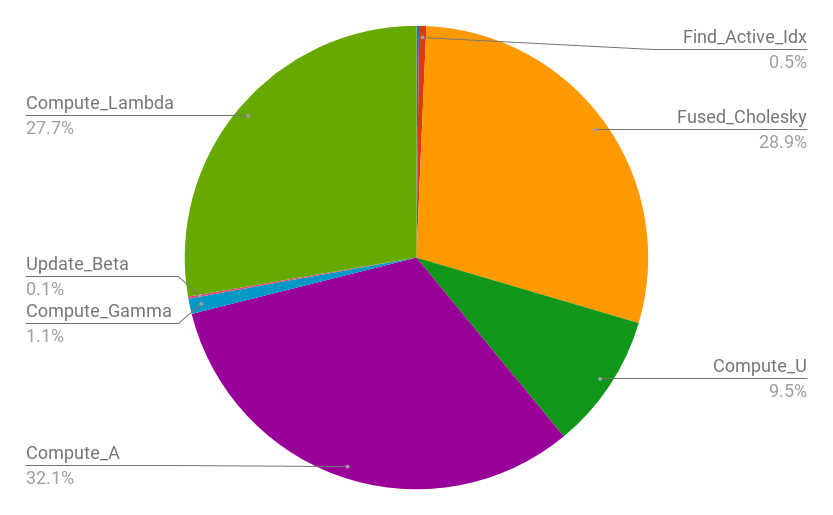
\includegraphics[scale=0.26]{./pic/pie_after.png}
  \caption{Run time after optimization}
  \label{fig:pie_after}
\end{figure}

\begin{figure}[h]
\centering
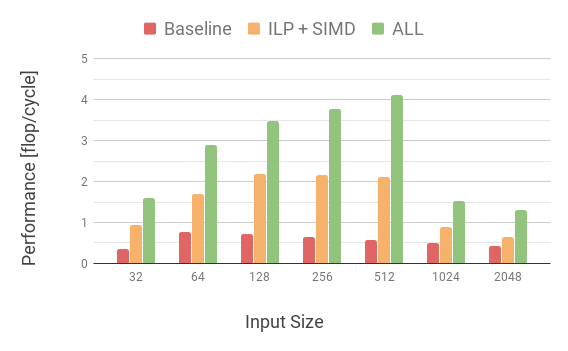
\includegraphics[width=0.5\textwidth]{./pic/performance.png}
\caption{Performance Comparison. \textsc{Baseline} is compiled w/o optimization flags, \textsc{ILP+SIMD} is baselin compiled with optimization falgs and \textsc{ALL} is our final optimized version.}
\label{fig:performance}
\end{figure}


As the input size increases, the overhead of optimization, such as extra branches for corner case of blocking and unrolling, become insignificant as the benefit grows faster. On the other hand, the performance and the speed-up gain drop dramatically on input sizes larger than 1024. One reason might be that for input size of 1024, the allocated memory space exceed the 8MB physical memory space. Then the run time is dominated by the access time of hard disk.


\begin{figure*}
\centering
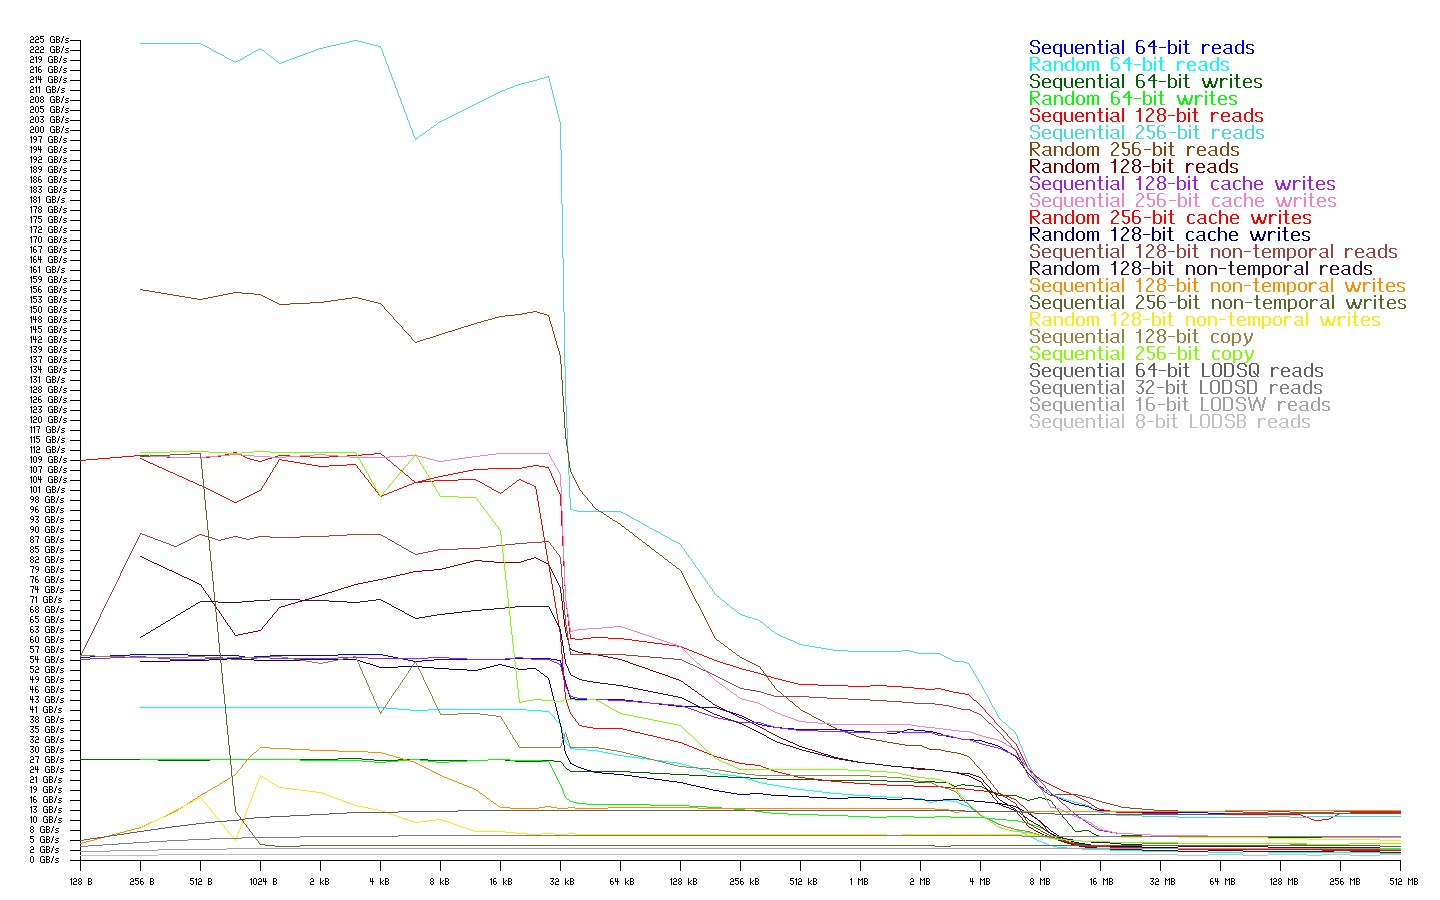
\includegraphics[scale=0.25]{./pic/bandwidth.jpg}
\caption{Measured memory bandwidth}
\label{fig:mem-bw}
\end{figure*}

The memory traffic is estimated as: 
$$
\# LLC\ misses \cdot LLC\ line\ size
$$
As argued by Georg Ofenbeck et al.\cite{ofenbeck2014applying} the actual traffic might be more than, even twice, the amount of observed LLC cache misses, depending on caching mechanism. Even though, it's still good upper bound of of memory traffic. Combining the measured memory traffic, measured run time cycles, and calculated floating point operation counts, we draw the roofline plot and examine the limitation of optimizing this algorithm.

\begin{figure}[h]
\centering
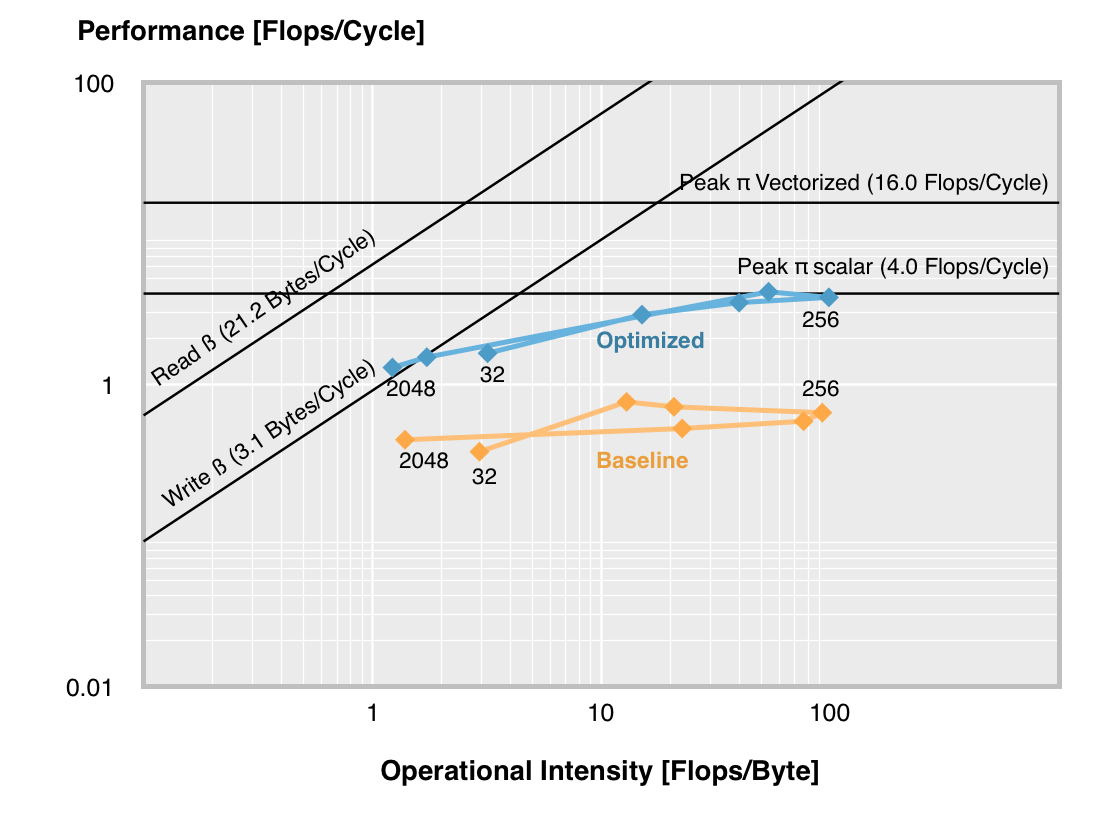
\includegraphics[width=0.5\textwidth]{./pic/roofline.png}
\caption{Roofline plot of baseline and optimized program.}
\label{fig:roofline}
\end{figure}

From the roofline plot in Figure~\ref{fig:roofline}, we know that the larger the input size is (larger than 256), the more likely the algorithm is memory bounded.





% Here you evaluate your work using experiments. You start again with a
% very short summary of the section. The typical structure follows.

% \mypar{Experimental setup} Specify the platform (processor, frequency, cache sizes)
% as well as the compiler, version, and flags used. I strongly recommend that you 
% play with optimization flags and consider also icc for additional potential speedup.

% Then explain what input you used and what range of sizes. The idea is to give 
% enough information so the experiments are reproducible by somebody else on his or her code.

% \mypar{Flags}
% -fma or/Qfma. If the instructions exist on the target processor, the compiler generates fused multiply-add (FMA) instructions.

% \mypar{Results}
% Next divide the experiments into classes, one paragraph for each. In the simplest
% case you have one plot that has the size on the x-axis and the performance on the
% y-axis. The plot will contain several lines, one for each relevant code version.
% Discuss the plot and extract the overall performance gain from baseline to best 
% code. Also state the percentage of peak performance for the best code. Note that
% the peak may change depending on the situation. For example, if you only do 
% additions it would be 12 Gflop/s
% on one core with 3 Ghz and SSE and single precision floating point.

% Do not put two performance lines into the same plot if the operations count 
% changed significantly (that's apples and oranges). In that case first perform 
% the optimizations that reduce op count and report the runtime gain in a plot. 
% Then continue to optimize the best version and show performance plots.

% {\bf You should}
% \begin{itemize}
% \item Follow the guide to benchmarking presented in class, in particular
% \item very readable, attractive plots (do 1 column, not 2 column plots
% for this class), proper readable font size. An example is below (of course you 
% can have a different style),
% \item every plot answers a question, which you pose and extract the
% answer from the plot in its discussion
% \end{itemize}
% Every plot should be discussed (what does it show, which statements do
% you extract).